\documentclass[12pt]{article}
\usepackage[hungarian]{babel}
\selectlanguage{hungarian}
\usepackage[utf8]{inputenc}
\usepackage[T1]{fontenc}

\pdfpageheight\paperheight
\pdfpagewidth\paperwidth
\setlength\topmargin{-1cm} \setlength\oddsidemargin{-0cm}
\setlength\textheight{24cm} \setlength\textwidth{15.8cm}
\setlength\columnsep{0.25in}  \newlength\titlebox \setlength\titlebox{2.00in}
\setlength\headheight{5pt}   \setlength\headsep{0pt}
\setlength\footskip{1cm}
\setlength\leftmargin{0.0in}

\usepackage{alltt}

\usepackage{tikz}
\usetikzlibrary{shapes,shapes.geometric,shapes.multipart,calc}
\tikzset{
  level distance=1cm, level 1/.style={sibling distance=3cm},
  level 2/.style={sibling distance=2cm},
  level 3/.style={sibling distance=1cm},
  treenode/.style = {align=center, inner sep=0pt, text centered, font=\sffamily},
  arn_n/.style = {treenode, circle, white, font=\sffamily\bfseries, draw=black, fill=black, text width=1.5em},
  arn_r/.style = {treenode, circle, white, draw=red, text width=1.5em, very thick, fill=red}
}
\usepackage{subfig}
\date{}
\title{4. gyakorlat -- Piros-fekete fa beszúrás}
\begin{document}

\maketitle

\noindent Emlékeztető: a piros-fekete fák olyan bináris keresőfák, amelyre teljesülnek az alábbiak:\\
--~A gyökér és minden levél színe fekete (amelyik csúcs nem fekete, az pedig piros)\\
--~A piros csúcsoknak \textbf{kizárólag} fekete színű gyerekeik vannak\\
--~Bármely csúcsból azonos számú fekete csúcs érintésével jutunk el bármelyik levélbe

\noindent1. Az alábbi fák közül melyekre teljesül a piros-fekete fákkal kapcsolatos összes elvárás?

\begin{figure}[!h]
\subfloat[Nem AVL fa]{
\begin{tikzpicture}
\node [arn_n] {54}
	child{ node [arn_r,sibling distance=2.2cm] {34}
		child{ node [arn_n] {9}
			child[missing]
			child{ node [arn_r]  {30}}
			}
		child{ node [arn_n] {50}
			child{ node [arn_r]  {49}}
			child[missing]
			}   
	}
	child{ node [arn_n] {75}
		child{ node [arn_r]  {68}
			child{ node [arn_r]  {56}}
			child[missing]
			}
		child{ node [arn_r] {98}}
	};
	\end{tikzpicture}
}~
\subfloat[Nem AVL fa]{
\begin{tikzpicture}
\node [arn_n] {54}
	child{ node [arn_r] {34}
		child{ node [arn_n] {9}
			child[missing]
			child{ node [arn_r]  {30}}
			}
		child{ node [arn_n] {50}
			child{ node [arn_r]  {49}}
			child[missing]
			}   
	}
	child{ node [arn_r] {75}
		child{ node [arn_n]  {68}
			child{ node [arn_r]  {56}}
			child[missing]
			}
		child[missing]
	};
	\end{tikzpicture}
}~
\subfloat[AVL fa]{
\begin{tikzpicture}
\node [arn_n] {54}
	child{ node [arn_r] {34}
		child{ node [arn_n] {9}
			child[missing]
			child{ node [arn_r]  {30}}
			}
		child{ node [arn_n] {50}
			child{ node [arn_r]  {49}}
			child[missing]
			}   
	}
	child{ node [arn_r] {75}
		child{ node [arn_n]  {68}
			child{ node [arn_r]  {56}}
			child[missing]
			}
		child{ node [arn_n]  {98}}
	};
	\end{tikzpicture}
}
\end{figure}

\noindent 2. Szúrjuk be az 55, 70, 7, 5, 69, 73 kulcsokat az előző feladat (c) jelű piros-fekete fájába.
% (9, 34, 50, 30, 54, 75, 49, 68, 98, 56)

\begin{figure}[!h]
\centering
\subfloat[fekete nagybácsi $\rightarrow$ forgatás]{
\begin{tikzpicture}
\node [arn_n] {54}
	child{ node [arn_r] {34}
		child{ node [arn_n] {9}
			child[missing]
			child{ node [arn_r]  {30}}
			}
		child{ node [arn_n] {50}
			child{ node [arn_r]  {49}}
			child[missing]
			}   
	}
	child{ node [arn_r] {75}
		child{ node [arn_n]  {56}
			child{ node [arn_r]  {55}}
			child{ node [arn_r]  {68}}
			}
		child{ node [arn_n]  {98}}
	};
	\end{tikzpicture}
}\\
\subfloat[piros nagybácsi $\rightarrow$ átszínezés(ek)]{
\begin{tikzpicture}
\node [arn_n] {54}
	child{ node [arn_n] {34}
		child{ node [arn_n] {9}
			child[missing]
			child{ node [arn_r]  {30}}
			}
		child{ node [arn_n] {50}
			child{ node [arn_r]  {49}}
			child[missing]
			}   
	}
	child{ node [arn_n] {75}
		child{ node [arn_r]  {56}
			child{ node [arn_n]  {55}}
			child{ node [arn_n]  {68}
				child[missing]
				child{ node [arn_r]  {70}}
			}
		}
		child{ node [arn_n]  {98}}
	};
	\end{tikzpicture}
}
\end{figure}
\begin{figure}[htb]\ContinuedFloat
\centering
\subfloat[fekete ős $\rightarrow$ nincs teendő]{
\begin{tikzpicture}
\node [arn_n] {54}
	child{ node [arn_n] {34}
		child{ node [arn_n] {9}
			child{ node [arn_r]  {7}}
			child{ node [arn_r]  {30}}
			}
		child{ node [arn_n] {50}
			child{ node [arn_r]  {49}}
			child[missing]
			}   
	}
	child{ node [arn_n] {75}
		child{ node [arn_r]  {56}
			child{ node [arn_n]  {55}}
			child{ node [arn_n]  {68}
				child[missing]
				child{ node [arn_r]  {70}}
			}
		}
		child{ node [arn_n]  {98}}
	};
	\end{tikzpicture}
}\\
\subfloat[piros nagybácsi $\rightarrow$ átszínezés]{
\begin{tikzpicture}
\node [arn_n] {54}
	child{ node [arn_n] {34}
		child{ node [arn_r] {9}
			child{ node [arn_n]  {7}
				child{ node [arn_r]  {5}}
				child[missing]
			}
			child{ node [arn_n]  {30}}
			}
		child{ node [arn_n] {50}
			child{ node [arn_r]  {49}}
			child[missing]
			}   
	}
	child{ node [arn_n] {75}
		child{ node [arn_r]  {56}
			child{ node [arn_n]  {55}}
			child{ node [arn_n]  {68}
				child[missing]
				child{ node [arn_r]  {70}}
			}
		}
		child{ node [arn_n]  {98}}
	};
	\end{tikzpicture}
}\\
\subfloat[fekete nagybácsi és zikk-zakk $\rightarrow$ 2~forgatás]{
\begin{tikzpicture}
\node [arn_n] {54}
	child{ node [arn_n] {34}
		child{ node [arn_r] {9}
			child{ node [arn_n]  {7}
				child{ node [arn_r]  {5}}
				child[missing]
			}
			child{ node [arn_n]  {30}}
			}
		child{ node [arn_n] {50}
			child{ node [arn_r]  {49}}
			child[missing]
			}   
	}
	child{ node [arn_n] {75}
		child{ node [arn_r]  {56}
			child{ node [arn_n]  {55}}
			child{ node [arn_n]  {69}
				child{ node [arn_r]  {68}}
				child{ node [arn_r]  {70}}
			}
		}
		child{ node [arn_n]  {98}}
	};
	\end{tikzpicture}
}\\
\subfloat[piros nagybácsi $\rightarrow$ kaszkád színezés]{
\begin{tikzpicture}
\node [arn_n] {54}
	child{ node [arn_n] {34}
		child{ node [arn_r] {9}
			child{ node [arn_n]  {7}
				child{ node [arn_r]  {5}}
				child[missing]
			}
			child{ node [arn_n]  {30}}
			}
		child{ node [arn_n] {50}
			child{ node [arn_r]  {49}}
			child[missing]
			}
	}
	child{ node [arn_n] {75}
		child{ node [arn_r]  {56}
			child{ node [arn_n]  {55}}
			child{ node [arn_r]  {69}
				child{ node [arn_n]  {68}}
				child{ node [arn_n]  {70}
					child[missing]
					child{ node [arn_r]  {73}}
				}
			}
		}
		child{ node [arn_n]  {98}}
	};
	\end{tikzpicture}
}~
\setcounter{subfigure}{5}
\subfloat[fekete nagybácsi és zikk-zakk $\rightarrow$ 2~forgatás]{
\begin{tikzpicture}
\node [arn_n] {54}
	child{ node [arn_n] {34}
		child{ node [arn_r] {9}
			child{ node [arn_n]  {7}
				child{ node [arn_r]  {5}}
				child[missing]
			}
			child{ node [arn_n]  {30}}
			}
		child{ node [arn_n] {50}
			child{ node [arn_r]  {49}}
			child[missing]
			}
	}
	child{ node [arn_n] {69}
		child{ node [arn_r]  {56}
			child{ node [arn_n]  {55}}
			child{ node [arn_n]  {68}}
		}
		child{ node [arn_r]  {75}
			child{ node [arn_n]  {70}
				child[missing]
				child{ node [arn_r]  {73}}
			}
			child{ node [arn_n]  {98}}			
		}
	};
	\end{tikzpicture}
}
\end{figure}

%b.) A beszúrások után kapott fából töröljük rendre a következő elemeket: 55, 98, 30, 50, 49, 7, 69, 5, 73, 75

\end{document}